\FloatBarrier
\section{Zero Moment Point}
\label{sec::21_zmp}
The key metric in this work, for the generation of a dynamically balanced gait, is the zero moment point. The concept was first introduced by Miomir Vukobratovi\'{c} and Davor Juri\v{c}i\'{c} in 1968 \cite{vukobratovic1968contribution}\cite{vukobratovic1969contribution} and first utilized in 1984 to generate walking trajectories for the WL-10RD robot \cite{yamaguchi1993development}. The most intuitive understanding for the ZMP arises by thinking about the realization of the simplest arbitrary possible walking motion for which a humanoid robot will not fall. This motion is achieved by ensuring the feet's whole area, and not only the edge, is in contact with the ground \cite{vukobratovic2004zero}, or put in other words, we require the robot not to rotate about its feet edges. This constraint can be met by having a reaction force $\bm{F}_r$ between the foot and the ground, which compensates for all external moments $\bm{M}_x$, and $\bm{M}_y$ around the x-, and y-axis at any time (fig. \ref{fig::21_zmp}).
\begin{figure}[h!]
	\centering
	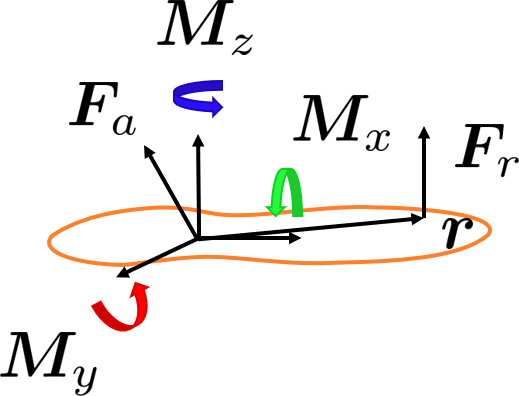
\includegraphics[scale=.5]{chapters/02_foundations_for_humanoid_walking/img/zero_moment_point.png}
	\caption{Forces, and moments that act on the foot. The support polygon is depicted by the orange line.}
	\label{fig::21_zmp}
\end{figure}
The point $\bm{r}$, at which the reaction force acts, is physically only meaningful if it lies within the foot's support polygon, that is the foot's area, which touches the ground (figure \ref{fig::21_zmp}). Not only can it not exist outside of the support polygon, since there was no point of interaction between the foot and the ground then, but also was the robot to overturn under these circumstances. Therefore, the ZMP is defined as that point on the ground at which the net moment of the inertial forces has no component along the horizontal axes \cite{hirai1998development}\cite{dasgupta1999making}. The knowledge of the zero moment point's location then allows one to control it, so to obtain dynamic balance. Its location depends, in principle, on all links, which are connected to the foot, and its computation may not be feasible for real-time applications. However, by simplifying a humanoid robot's physics as a linear inverted pendulum, one obtains a simple analytic relationship between the robot's center of mass and its zero moment point, which is described in following section - Zero Moment Point of a Linear Inverted Pendulum.
\FloatBarrier
\subsection{Zero Moment Point of a Linear Inverted Pendulum}
Dynamically balanced walking trajectories can be generated by simplifying the dynamics of humanoid robots to those of a linear inverted pendulum \cite{kajita2003biped}. A rigorous derivation for the analytic relation between the center of mass and the zero moment point of a linear inverted pendulum exists in \cite{kajita2014introduction}, but for the sake of simplicity we rather explain the physics in terms of cutting forces, for which a short introduction is in the summary of the lecture Robotics 1 (\href{https://drive.google.com/file/d/1aN1ujXTOlHzO2kLPK7TQRkWfdY-pGzUF/view}{\underline{link}}). 
\begin{figure}[h!]
	\centering
	\subcaptionbox{}%
	[.4\linewidth]{
\includegraphics[scale=.3]{chapters/02_foundations_for_humanoid_walking/img/inverted_pendulum.png}}
	\subcaptionbox{}%
	[.4\linewidth]{
\includegraphics[scale=.3]{chapters/02_foundations_for_humanoid_walking/img/inverted_pendulum_free_body_diagram.png}}
	\caption{Linear inverted pendulum with a support polygon (a), and the corresponding free body diagram with cutting forces $\bm{S}_{x/y/z}$ (b).}
	\label{fig::21_lip}
\end{figure}
The system of interest is shortly depicted in figure \ref{fig::21_lip}. We assume the support polygon of the shown linear inverted pendulum to be rectangular, and to have zero mass. By introducing cutting forces $\bm{S}_{x/y/z}$ for each degree of freedom in which the motion of the linear inverted pendulum is restricted, we obtain the free body diagram (fig. \ref{fig::21_lip}), for which the acting forces are
\begin{align}
	m\ddot{\bm{c}} &=\quad\bm{S} - \bm{F}_g 
	\label{eq::21_pendulum_force} \\
	\bm{0} &= -\bm{S}+\bm{F}_r
	\label{eq::21_support_polygon_force}
\end{align}
where $\bm{S}=\bm{S}_x+\bm{S}_y+\bm{S}_z$. The respective moments, since we do not take any inertias into account, are given by
\begin{align}
	\bm{0} &= (\bm{0}-\bm{c})\times\bm{S} + \bm{M} 
	\label{eq::21_pendulum_moment}\\	
	\bm{0} &= (\bm{r}-\bm{0})\times\bm{F}_r - \bm{M}
	\label{eq::21_support_polygon_moment}	
\end{align}
where the transfer of the moment $\bm{M}$ may for example be induced by friction. If we replace $\bm{S}=\bm{F}_r$ from eq. \ref{eq::21_support_polygon_force}, equations \ref{eq::21_pendulum_moment} and \ref{eq::21_support_polygon_moment} yield 
\begin{align}
	\bm{0} = (\bm{r}-\bm{c})\times\bm{S} = \begin{pmatrix}
	\quad(r_y - c_y)S_z - (r_z - c_z)S_y \\
	-(r_x - c_x)S_z + (r_z - c_z)S_x \\
	\quad(r_x - c_x)S_y - (r_y - c_y)S_x
	\end{pmatrix}
	\label{eq::21_momentum_transfer}
\end{align}
Since our goal is to have a robot that does not fall, we want to achieve that the acceleration along the z-axis becomes zero, hence $\ddot{c}_z=0$. Given this assumption, we can infer from eq. \ref{eq::21_pendulum_force} that $S_z=mg$, as well as $S_x = \ddot{c}_xm$, and $S_y = \ddot{c}_ym$. Furthermore, our foot shall not lift off the floor, and therefore we have $r_z=0$. If we take these assumptions and plug them into the first to rows of eq. \ref{eq::21_momentum_transfer}, we find
\begin{align}
	r_x &= c_x - c_z\frac{\ddot{c}_x}{g}
	\label{eq::211_zmp_x}\\
	r_y &= c_y - c_z\frac{\ddot{c}_y}{g}
	\label{eq::211_zmp_y}
\end{align}
Therein, $r_x$, and $r_y$ are the x-, and y-coordinates of the zero moment point, given the assumption of a linear inverted pendulum. One can see that the position is dependent on the height of the point mass, which is, in turn, dependent on the robot. Equations \ref{eq::211_zmp_x}, and \ref{eq::211_zmp_y} now give a simple analytic relationship between the zero moment point and the center of mass, which will helps to formulate an optimal control problem for humanoid walking that can be solved in real-time (section \ref{sec::22_nmpc}). This simplification is, of course, only true to some extent, and one needs to find a way to verify its accuracy. The easiest way to do so is to measure the real zero moment point, which will be further elaborated on within the next section - Measurement of the Zero Moment Point.
\FloatBarrier
\subsection{Measurement of the Zero Moment Point}
There exist several methods that enable one to measure the position of the zero moment point, among them the utilization of pressure-sensitive soles, as outlined in \cite{kajita2014introduction}. Furthermore, there exist approximate approaches that involve the knowledge of all acting external forces \cite{huang2001planning}, which can, for example, be obtained from unconstrained inverse dynamics \cite{michel2017dynamic}. However, measurements with force-torque sensors that are located at the ankles, also allow to infer the position of the zero moment point \cite{kajita2014introduction}, which is of special interest to this thesis.
\begin{figure}[h!]
	\centering
	
\includegraphics[scale=.5]{chapters/02_foundations_for_humanoid_walking/img/ft_sensor.png}
	\caption{Force-torque sensors at the foot's ankle.}
	\label{fig::21_force_torque}
\end{figure}
If one considers the force-torque sensor to be located at position $\bm{p}_i$ (fig. \ref{fig::21_force_torque}), then one can obtain the moment about any point $\bm{p}$ according to eq. \ref{eq::21_moment}.
\begin{align}
	\bm{\tau}(\bm{p}) = (\bm{p}_i-\bm{p})\times \bm{f}_i + \bm{\tau}_i
	\label{eq::21_moment}
\end{align}
by definition, the moment about the zero moment point vanishes along the horizontal axes, therefore one can set $\tau_x = \tau_y = 0$ in eq. \ref{eq::21_moment} and then solve for the position to obtain the zero moment point (eq. \ref{eq::21_x_pos_zmp} and \ref{eq::21_y_pos_zmp}).
\begin{align}
	p_x &= \frac{\left[-\tau_{i,y}-(p_{i,z}-p_z)f_{i,x}+p_{i,x}f_{i,z}\right]}{f_{i,z}}
	\label{eq::21_x_pos_zmp}\\
	p_y &= \frac{\left[-\tau_{i,x}-(p_{i,z}-p_z)f_{i,y}+p_{i,y}f_{i,z}\right]}{f_{i,z}}
	\label{eq::21_y_pos_zmp}
\end{align}
If one further chooses the coordinate system to lie along the force-torque sensor's z-axis, one can simplify equations \ref{eq::21_x_pos_zmp} and \ref{eq::21_y_pos_zmp} to find
\begin{align}
	p_x &= \frac{(-\tau_{i,y}-f_{1,x}d)}{f_{1,z}} 
	\label{eq::21_x_pos_zmp_simp}\\
	p_y &= \frac{(\tau_{i,x}-f_{1,y}d)}{f_{1,z}}
	\label{eq::21_y_pos_zmp_simp}
\end{align}
One can use equations \ref{eq::21_x_pos_zmp_simp} and \ref{eq::21_y_pos_zmp_simp} to determine the position of the zero moment point for the left and the right foot with respect to coordinates frames that are attached to the respective foot. These circumstances change once not only one, but both feet are in contact with the ground. What still holds true, in the case of a dynamically balanced gait, is the fact that the positions which one just obtained from equations \ref{eq::21_x_pos_zmp_simp} and \ref{eq::21_y_pos_zmp_simp} represent points where the interaction of the robot with the environment can solely be described by a single force along the z-axis. All other forces or torques cancel out. Therefore, to determine the position of the zero moment point for the double support phase, one needs to modify equation \ref{eq::21_moment} slightly. This yields 
\begin{align}
	\bm{\tau}(\bm{p}) = \sum_{i\in\{L, R\}} (\bm{p}_i - \bm{p})\times\bm{f}_i
	\label{eq::21_moment_ds}
\end{align}
where the individual torques are now zero and the only forces $\bm{f}_i$ that exist between the robot and the environment can be described by the z-components which are measured at the ankles' force-torque sensors. Yet again, to obtain the position of the zero moment point, one has to set the x-, and y-components of the torque in equation \ref{eq::21_moment_ds} to zero and find
\begin{align}
	p_x &= \frac{\sum_{i\in\{L, R\}}p_{i,x}f_{i,z}}{\sum_{i\in\{L, R\}}f_{i,z}} \\
	p_y &= \frac{\sum_{i\in\{L, R\}}p_{i,y}f_{i,z}}{\sum_{i\in\{L, R\}}f_{i,z}}
\end{align}
These expressions of course only hold true in a shared coordinate system and therefore one needs to transform the position of the zero moment point, which were obtained from equations \ref{eq::21_x_pos_zmp_simp} and \ref{eq::21_y_pos_zmp_simp}, to the world frame. Finally, one can write down the formulation for the zero moment point, which holds equally true for the single and double support phase
\begin{align}
	p_x &= \frac{p_{R,x}f_{R,z}+p_{L,x}f_{L,z}}{f_{R,z}+f_{L,z}} 
	\label{eq::21_double_zmp_x} \\
	p_y &= \frac{p_{R,y}f_{R,z}+p_{L,y}f_{L,z}}{f_{R,z}+f_{L,z}}
	\label{eq::21_double_zmp_y}
\end{align}
At this point one is now equipped with a general understanding for the zero moment point, as well as with the knowledge of simplified models to compute it analytically, and a method to measure it so that one can evaluate the performance of a potential pattern generator which is based upon the zero moment point. Therefore, the next chapter - Nonlinear Model Predictive Control, explains a method that allows one to generate dynamically balanced center of mass and feet trajectories, which satisfy the just introduced concepts optimally.
